\documentclass[12pt,a4paper]{article}
\usepackage[utf8]{vietnam}
\usepackage[left=1.5cm, right=1.5cm, top=1.5cm, bottom=2cm]{geometry}
\usepackage{graphicx}
\usepackage{mathtools}
\usepackage{amssymb}
\usepackage{amsthm}
\usepackage{nameref}
\usepackage{amsmath}
\usepackage{amsfonts}
\usepackage{enumitem}

\usepackage{pgfplots}
\pgfplotsset{compat=1.15}
\usepackage{mathrsfs}
\usetikzlibrary{arrows}
\pagestyle{empty}

\definecolor{uuuuuu}{rgb}{0.26666666666666666,0.26666666666666666,0.26666666666666666}

\begin{document}

\begin{center}
	\textbf{\underline{{\Large Chứng minh định lý Brocard bằng kiến thức THCS}}}\\
\end{center}

\textbf{Phát biểu định lý:} Cho tứ giác toàn phần BADCXY nội tiếp đường tròn (O); Z là giao điểm của AC, DB. Chứng minh rằng: O là trực tâm của tam giác XYZ.\\




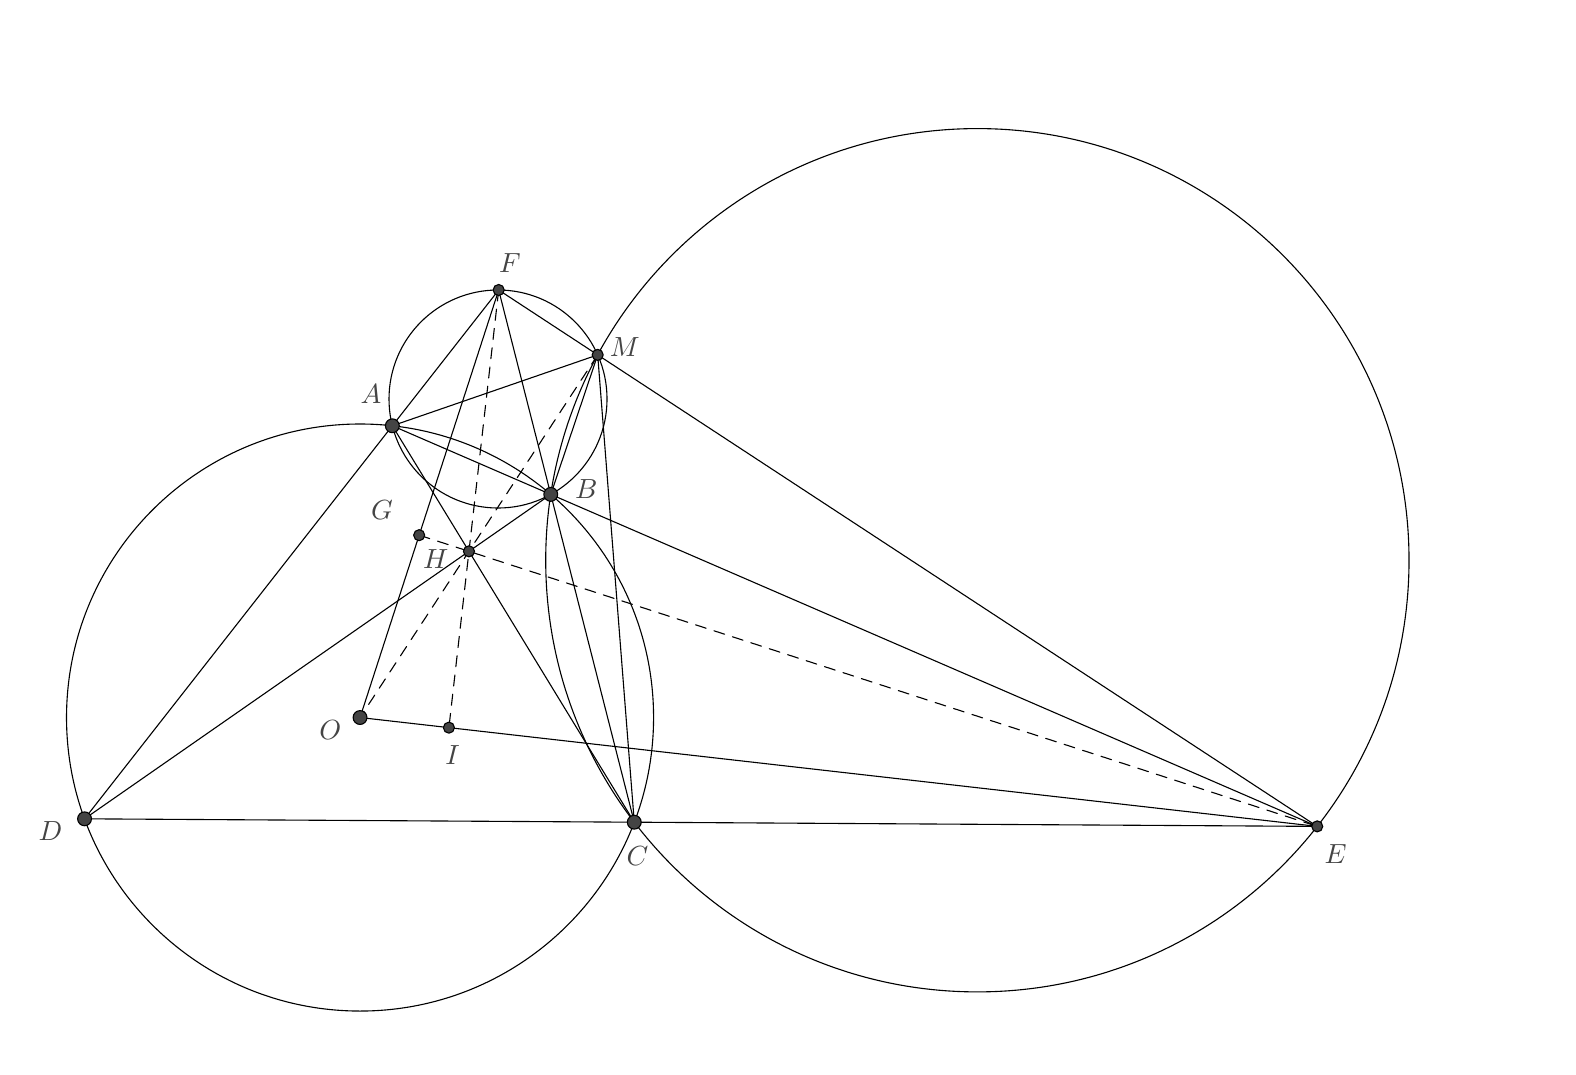
\begin{tikzpicture}[line cap=round,line join=round,>=triangle 45,x=1cm,y=1cm]
	\clip(-5.75119863572696,-3.419600353577202) rectangle (13.560756218837444,9.521197365887557);
	\draw   (-1.1198412799266677,4.465108187346908)-- (1.952704122239836,-0.5692211450811859);
	\draw   (0.8920317919726709,3.5936935004108923)-- (-5.028756998508487,-0.5263733210017867);
	\draw   (0.23062348648099065,6.189581262362677)-- (-1.53,0.76);
	\draw   (-1.53,0.76)-- (10.626032037482737,-0.6224525850717072);
	\draw   (10.626032037482737,-0.6224525850717072)-- (0.23062348648099065,6.189581262362677);
	\draw   (0.23062348648099065,6.189581262362677)-- (1.952704122239836,-0.5692211450811859);
	\draw   (0.23062348648099065,6.189581262362677)-- (-5.028756998508487,-0.5263733210017867);
	\draw   (-1.1198412799266677,4.465108187346908)-- (10.626032037482737,-0.6224525850717072);
	\draw   (-5.028756998508487,-0.5263733210017867)-- (10.626032037482737,-0.6224525850717072);
	\draw  (-1.53,0.76) circle (3.727741522101188cm);
	\draw [dash pattern=on 4pt off 3pt] (1.4880253477553584,5.3656151818758655)-- (-1.53,0.76);
	\draw (6.309949043193097,2.757546846132009) circle (5.482058789226331cm);
	\draw (0.2221270985820833,4.805212206116102) circle (1.3843951287476999cm);
	\draw [dash pattern=on 4pt off 3pt] (0.23062348648099065,6.189581262362677)-- (-0.40145520442875066,0.6316555151223695);
	\draw [dash pattern=on 4pt off 3pt] (-0.7790603707396485,3.0758203735808247)-- (10.626032037482737,-0.6224525850717072);
	\draw   (1.4880253477553584,5.3656151818758655)-- (0.8920317919726709,3.5936935004108923);
	\draw   (1.4880253477553584,5.3656151818758655)-- (1.952704122239836,-0.5692211450811859);
	\draw   (1.4880253477553584,5.3656151818758655)-- (-1.1198412799266677,4.465108187346908);
	\begin{scriptsize}
		\draw [fill=uuuuuu] (-1.53,0.76) circle (2.5pt);
		\draw[color=uuuuuu] (-1.9076933607771975,0.6000009302585) node {\normalsize$O$};
		\draw [fill=uuuuuu] (0.8920317919726709,3.5936935004108923) circle (2.5pt);
		\draw[color=uuuuuu] (1.3419965551457308,3.659673767787805) node {\normalsize$B$};
		\draw [fill=uuuuuu] (-1.1198412799266677,4.465108187346908) circle (2.5pt);
		\draw[color=uuuuuu] (-1.3897384639156807,4.867565238360825) node {\normalsize$A$};
		\draw [fill=uuuuuu] (1.952704122239836,-0.5692211450811859) circle (2.5pt);
		\draw[color=uuuuuu] (1.9939246720187733,-0.9998540587311804) node {\normalsize$C$};
		\draw [fill=uuuuuu] (-5.028756998508487,-0.5263733210017867) circle (2.5pt);
		\draw[color=uuuuuu] (-5.463328307250099,-0.67989634292351013) node {\normalsize$D$};
		\draw [fill=uuuuuu] (10.626032037482737,-0.6224525850717072) circle (2pt);
		\draw[color=uuuuuu] (10.861038113452964,-0.96991748501967494) node {\normalsize$E$};
		\draw [fill=uuuuuu] (0.23062348648099065,6.189581262362677) circle (2pt);
		\draw[color=uuuuuu] (0.37408394247654203,6.533397511064584) node {\normalsize$F$};
		\draw [fill=uuuuuu] (1.4880253477553584,5.3656151818758655) circle (2pt);
		\draw[color=uuuuuu] (1.8339570898995581,5.461479260503088) node {\normalsize$M$};
		\draw [fill=uuuuuu] (-0.14680675572277027,2.8708026180261657) circle (2pt);
		\draw[color=uuuuuu] (-0.5698230323003365,2.7787667930109305) node {\normalsize$H$};
		\draw [fill=uuuuuu] (-0.7790603707396485,3.0758203735808247) circle (2pt);
		\draw[color=uuuuuu] (-1.2497525586464566,3.397713233033979) node {\normalsize$G$};
		\draw [fill=uuuuuu] (-0.40145520442875066,0.6316555151223695) circle (2pt);
		\draw[color=uuuuuu] (-0.35384276492342287,0.2860064034341317) node {\normalsize$I$};
	\end{scriptsize}
\end{tikzpicture}




\end{document}